%%% PREAMBLE

\documentclass{article}
\usepackage{amsmath,amssymb,amsthm,fullpage,graphicx,subcaption}

% Use break between paragraphs instead of indentation
%\usepackage{parskip}

% Code highlighting
\usepackage[utf8]{inputenc}
\usepackage{listings, color}

% Default fixed font does not support bold face
\DeclareFixedFont{\ttb}{T1}{txtt}{bx}{n}{9} % for bold
\DeclareFixedFont{\ttm}{T1}{txtt}{m}{n}{9}  % for normal

% Custom colors
\usepackage{color}
\definecolor{deepblue}{rgb}{0,0,0.5}
\definecolor{deepred}{rgb}{0.6,0,0}
\definecolor{deepgreen}{rgb}{0,0.5,0}

% Python style for highlighting
\newcommand\pythonstyle{\lstset{
language=Python,
basicstyle=\ttm,
otherkeywords={self},             % Add keywords here
keywordstyle=\ttb\color{deepblue},
emph={MyClass,__init__},          % Custom highlighting
emphstyle=\ttb\color{deepred},    % Custom highlighting style
stringstyle=\color{deepgreen},
frame=tb,                         % Any extra options here
showstringspaces=false,           % 
commentstyle=\ttm\color{magenta}
}}

% Python environment
\lstnewenvironment{python}[1][]
{
\pythonstyle
\lstset{#1}
}
{}

% Python for external files
\newcommand\pythonex[2][]{{
\pythonstyle
\lstinputlisting[#1]{#2}}}

% Python for inline
\newcommand\pyln[1]{{\pythonstyle\lstinline!#1!}}

% Various math conveniences
\theoremstyle{definition}
\newtheorem*{prop}{Proposition}
\newtheorem*{obs}{Observation}
\newtheorem*{lemma}{Lemma}
\newtheorem*{disc}{Discussion}
\newtheorem*{qn}{Question}
\renewcommand{\bar}{\overline}
\newcommand{\nin}{\not\in}
\renewcommand{\>}{\rangle}
\newcommand{\<}{\langle}



%%% FILE INFO

% Header
%\usepackage{fancyhdr}
%\usepackage[margin=1in, headheight=50pt]{geometry}
%\pagestyle{fancy}
%\lhead{\textbf{CS21}}
%\chead{Final}
%\rhead{Aritra Biswas}
%\setlength{\headsep}{20pt}

% Title stuff
\title{\textbf{Set 2: Numerical Integration}}
\date{}
\author{Aritra Biswas}



%%% DOCUMENT

\begin{document}

\maketitle

\section{Simpson's formula}

We show that Simpson's formula for the integral
$I=\int_a^b f(x) dx$ has a local error of $O(H^5)$ with $H=b-a$. We can
express $f(x)$ as a Taylor series around $x=a$:
\begin{align}\label{eqn:taylor}
f(x) = f(a) + f'(a)(x-a) + \frac{f''(a)}{2!}(x-a)^2
+ \frac{f^{(3)}(a)}{3!}(x-a)^3
+ \frac{f^{(4)}(\eta)}{4!}(x-a)^4,
\end{align}
with $x,\eta\in[a,b]$. Integrating from $a$ to $b$, we obtain:
\begin{align*}
I = f(a)H + f'(a)\frac{H^2}{2!} + f''(a)\frac{H^3}{3!} +
f^{(3)}(a)\frac{H^4}{4!} + f^{(4)}(\eta)\frac{H^5}{5!}.
\end{align*}
Using equation \ref{eqn:taylor} to estimate $f(b)$ and $f(c)$, we can
rearrange Simpson's formula:
\begin{align*}
I_{simp} &= \frac{H}{6}f(a) + \frac{4H}{6}f(c) + \frac{H}{6}f(b) \\
&= \frac{H}{6}f(a) 
+ \frac{4H}{6}\left(f(a) + f'(a)\frac{H}{2} + \frac{f''(a)}{2!}\left(\frac{H}{2}\right)^2
+ \frac{f^{(3)}(a)}{3!}\left(\frac{H}{2}\right)^3
+ \frac{f^{(4)}(\eta)}{4!}\left(\frac{H}{2}\right)^4\right) \\
&\;\;\;\;+ \frac{H}{6}\left(
f(a) + f'(a)H + \frac{f''(a)}{2!}H^2
+ \frac{f^{(3)}(a)}{3!}H^3
+ \frac{f^{(4)}(\eta)}{4!}H^4\right) \\
&= \frac{H}{6}f(a) 
+ \frac{4H}{6}\left(f(a) + f'(a)\frac{H}{2} + \frac{f''(a)}{2!}\frac{H^2}{4}
+ \frac{f^{(3)}(a)}{3!}\frac{H^3}{8}
+ \frac{f^{(4)}(\eta)}{4!}\frac{H^4}{16}\right) \\
&\;\;\;\;+ \frac{H}{6}\left(
f(a) + f'(a)H + \frac{f''(a)}{2!}H^2
+ \frac{f^{(3)}(a)}{3!}H^3
+ \frac{f^{(4)}(\eta)}{4!}H^4\right) \\
&= f(a)H + f'(a)\left(\frac{4H^2}{6\cdot2}+\frac{H^2}{6}\right)
+ f''(a)\left(\frac{4H^3}{6\cdot2!\cdot4} + \frac{H^3}{6\cdot2!}\right)
+ f^{(3)}(a)\left(\frac{4H^4}{6\cdot3!\cdot8}+\frac{H^4}{6\cdot3!}\right) \\
&\;\;\;\;+ f^{(4)}(\eta)\left(\frac{4H^5}{6\cdot4!\cdot16}+\frac{H^5}{6\cdot4!}\right) \\
&= f(a)H + f'(a)\frac{H^2}{2!} + f''(a)\frac{H^3}{3!}
+ f^{(3)}(a)\frac{H^4}{4!} + f^{(4)}(\eta)\frac{5H^5}{576}.
\end{align*}
This gives the error:
\begin{align*}
I - I_{simp} &= -\frac{H^5}{2880}f^{(4)}(\eta) = O(H^5).
\end{align*}

When we divide the interval $[a,b]$ into $N$ subintervals of width
$h_N=(b-a)/N$, we obtain the extended Simpson's formula. Let
$x_i = a + ih_N$, and let $m_{i,j}=\frac{x_i + x_j}{2}$.
\begin{align*}
\int_a^b f(x)dx &= \int_{x_0}^{x_1}f(x)dx + \int_{x_1}^{x_2}f(x)dx
+ \cdots \int_{x_{N-1}}^{x_N}f(x)dx \\
&\approx h_N\left(\frac{f(x_0)+4f(m_{0,1})+f(x_1)}{6}\right)
+ h_N\left(\frac{f(x_1)+4f(m_{1,2})+f(x_2)}{6}\right) + \cdots \\
&\;\;\;\;+ h_N\left(\frac{f(x_{N-1})+4f(m_{N-1,N})+f(x_N)}{6}\right)\\
&= {h_N}\left(\frac{f(x_0)+4f(m_{0,1})+2f(x_1)+4f(m_{1,2})+2f(x_2)
+\cdots+2f(x_{N-1})+4f(m_{N-1,N})+f(x_N)}{6}\right).
\end{align*}

The global error is the local error multiplied by the number of subintervals:
\begin{align*}
-\frac{h_N^5}{2880}f^{(4)}(\eta)\cdot N = -\frac{h_N^5}{2880}f^{(4)}(\eta)
\cdot\frac{b-a}{h_N} = O(h_N^4).
\end{align*}

\section{Implementation of trapezoidal method}

\pythonex[firstline=14, lastline=39]{defint.py}

\newpage
\section{Implementation of Simpson's method}

\pythonex[firstline=41, lastline=69]{defint.py}

\section{Comparison of trapezoidal and Simpson's methods}

\begin{figure}\centering
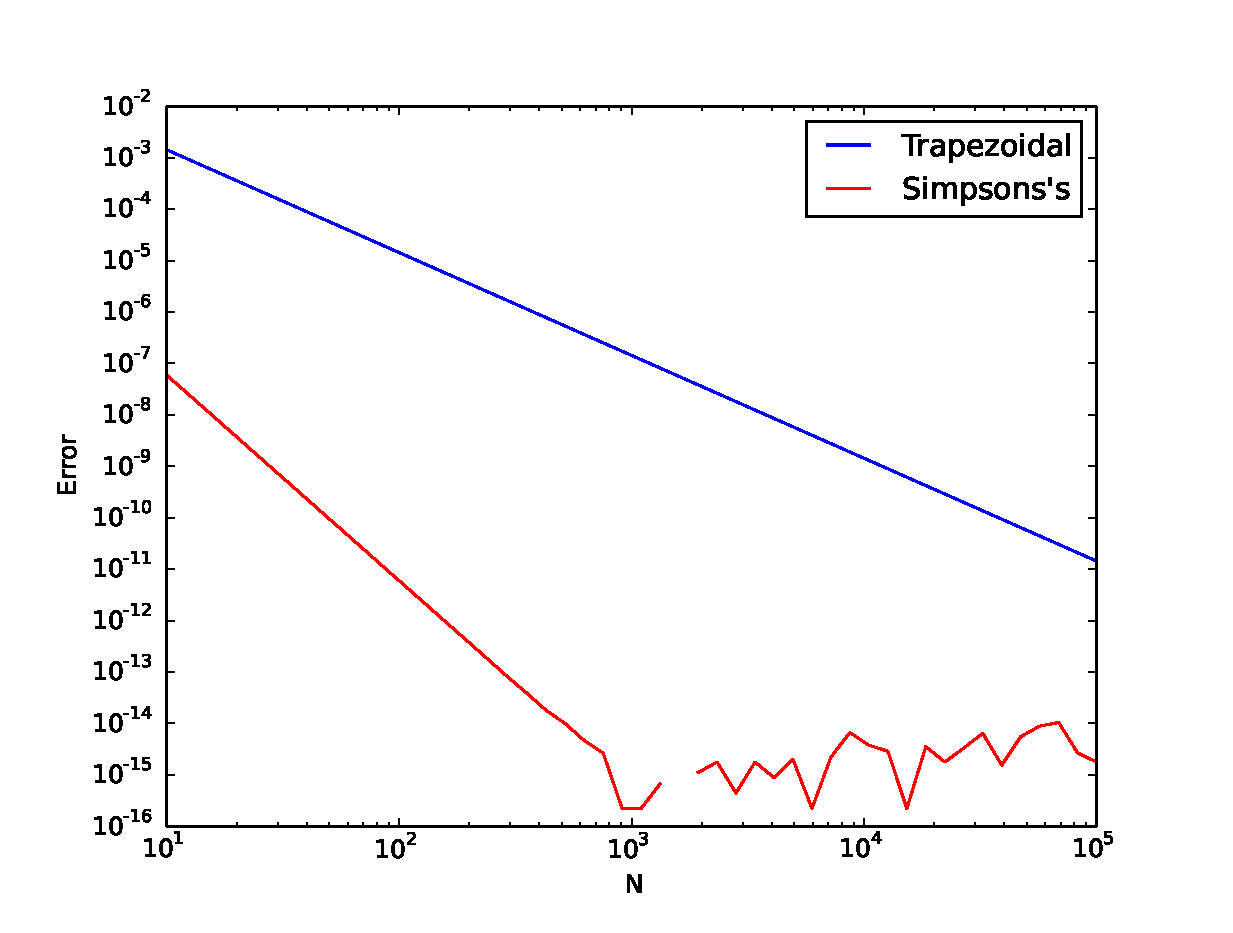
\includegraphics[width=\textwidth]{convergence.eps}
\caption{\label{fig:convergence}Convergence plot showing the errors of the trapezoidal method
and Simpson's method on the same scale.}
\end{figure}

We use each of the above functions to evaluate $\int_0^1 e^x dx$ with $N$
ranging from 10 to $10^5$. Figure \ref{fig:convergence} shows the convergence
plot for both methods on the same scale, plotting the error against the
expected value 1.7182818284590452354.

Clearly, Simpson's method is much more accurate at low $N$. Furthermore,
Simpson's method exhibits some odd behavior at very large values of $N$:
the error tends to oscillate. Our plotting subroutine compares the
computed value of the integral with the given exact value, and when
this difference is very low (i.e. lower than $10^{-12}$ or $10^{-13}$)
we expect the subtraction to yield bogus answers due to roundoff error.

\newpage
\section{Simpson's method to desired accuracy}

We write a routine to integrate a function using Simpson's method repeatedly,
starting with a predefined $N=N_0$, and doubling $N$ each time until the
relative difference between succesive approximations is less than the requested
accuracy.
\pythonex[firstline=100, lastline=119]{defint.py}

We use this subroutine to calculate the integrals:
\begin{align*}
\int_0^1 e^x dx \text{ and } \int_1^2 x\sin\left(\frac{1}{x^2}\right)dx. \\
\end{align*}
Since \pyln{simps_ac} simply runs the \pyln{simps} routine until the desired relative accuracy is
obtained, the calculated value from \pyln{simps_ac} is the same as the value that \pyln{simps}
would return for the corresponding value of $N$.

The routine checks relative accuracy, so higher values of \pyln{ac} will require many more iterations
of Simpson's method. Since the desired accuracy is already provided, an interesting metric for this
funtion's performance is the time required to calculate integrals to various values of \pyln{ac}. All times
are total CPU times reported by IPython's \pyln{time} profiling.

\begin{table}[h!]\centering
\begin{tabular}{l | l | l}
Accuracy \pyln{ac} & Time for $\int_0^1 e^x dx$ & Time for $\int_1^2 x\sin\left(\frac{1}{x^2}\right)dx$ \\
\hline\hline
$10^{-5}$ & 3.33 ms & 3.33 ms \\
$10^{-10}$ & 6.67 ms & 10 ms \\
$10^{-13}$ & 13.3 ms & 26.7 ms \\
$10^{-15}$ & 36.7 ms & 2.38 s \\
\end{tabular}
\end{table}

The routine can take a considerable amount of time to run at high accuracy, especialy
when the function being integrated is rapidly changing, like $x\sin\left(\frac{1}{x^2}\right)$.

\newpage
\section{SciPy integration functions}

As expected, \pyln{scipy.integrate.quad} and \pyln{scipy.integrate.romberg} are much faster
in obtaining similar degrees of accuracy. We use these methods to calculate the two integrals
in Section 5. In many cases, IPython reports a CPU time of 0 ns, i.e. too quick to measure
accurately.

\begin{table}[h!]\centering
\begin{tabular}{l | l | l}
Measure & $\int_0^1 e^x dx$ & $\int_1^2 x\sin\left(\frac{1}{x^2}\right)dx$ \\
\hline\hline
\pyln{quad} value & 1.7182818284590453 & 0.6551059188460544 \\
\pyln{quad} error bound & 1.9076760487502457 $\times 10^{-14}$ & 7.27313674671109 $\times 10^{-15}$ \\
\pyln{quad} time & 0 ns & 0 ns \\
\hline
\pyln{romberg} value & 1.7182818284590782 & 0.65495874492202644 \\
\pyln{romberg} time & 0 ns & 13.3 ms \\
\end{tabular}
\end{table}

\end{document}
